\documentclass{article}
\usepackage[T1]{fontenc}
\usepackage{microtype}
\usepackage{graphicx}
\usepackage{booktabs}
\usepackage{multirow}
\usepackage{amsmath,amssymb}
\usepackage{xcolor}
\usepackage{hyperref}
\usepackage[accepted]{icml2026}   % swap for icml2026 (review) before submission; icml2027 when released
\graphicspath{{../figures/}}
\newcommand{\ir}[1]{\input{../tables/#1}}
\newcommand{\todo}[1]{\textcolor{red}{[#1]}}

\icmltitlerunning{Consistency, Not Plausibility}

\begin{document}
\twocolumn[
\icmltitle{Consistency, Not Plausibility: Dissociating Detection from Correction\\of Corrupted Tool Records in Scientific LLM Agents}
\icmlsetsymbol{equal}{*}
\begin{icmlauthorlist}
\icmlauthor{George Xu}{hms}
\end{icmlauthorlist}
\icmlaffiliation{hms}{Harvard Medical School and Massachusetts General Hospital, Boston, MA, USA}
\icmlcorrespondingauthor{George Xu}{}
\icmlkeywords{tool use, agents, knowledge conflicts, scientific agents, evaluation}
\vskip 0.3in
]
\printAffiliationsAndNotice{}

\begin{abstract}
Agents that answer scientific questions through database tools inherit whatever the tools return, and a well-formed record with a wrong value carries no signal that anything is amiss. We ask whether such agents apply domain plausibility checks to tool output, and whether noticing a bad value changes what they answer. An agent answers factual questions about proteins or small molecules through mock lookup tools backed by real UniProt and PubChem records; in corrupted conditions one task-relevant field is silently replaced by a value that is either impossible (a 3-residue, 58\,kDa protein; a molecule of 2\,Da; $-3$ hydrogen-bond donors) or plausible but wrong. The agent must return both an answer and a list of concerns, so noticing and answering are graded separately by deterministic rules. Across ten models from five vendors, two domains and roughly 22{,}000 runs, impossible values are flagged in the concerns in 75--100\% of runs yet still appear in the final answer in 32--93\%; plausible corruptions propagate in 93--100\% of runs whether they shrink or inflate the value, and the ordering of models is the same in both domains (Spearman $\rho=0.71$). Three manipulations show what drives the correction that does occur. A severity sweep that keeps the record internally consistent propagates at 80--100\% down to a 200-fold error for every model, whereas an inconsistent record is partly repaired from the intact field. A rule-based classifier over 2{,}700 flagged concerns finds that flags citing a repairable contradiction precede correction and flags citing bare implausibility do not, and that vendors differ in which cues their models cite. Replacing the compact summary record with the full database entry eliminates propagation of impossible values for every field the record can derive (organism errors $100\%\to0\%$ in UniProt; 0 of 75 numeric errors in PubChem) and leaves fields with no derivation route unchanged. Chemistry, where molecular formulas are well memorised, sharpens the picture: models detect 20\% errors in up to 96\% of runs and still relay them in 98\%, overriding the tool only when a check is decisive. A one-sentence sanity-check instruction cuts propagation of impossible values to 4--22\% for seven of the ten models. Code, data, traces and grading scripts are released.

\end{abstract}

\section{Introduction}
\label{sec:intro}

Agentic systems for the sciences act on what their tools return. A copilot that answers a question about a protein, a planner that chooses a perturbation, or a closed-loop system that schedules an assay pulls records from databases such as UniProt \citep{uniprot2025} or PubChem \citep{kim2025pubchem} and reasons from them \citep{huang2025biomni,roohani2024biodiscovery,fa2026bioagent,bran2024chemcrow}. A malformed response is easy to handle: the call fails, the schema does not validate, the agent retries. A well-formed record with a wrong value is not. Nothing in the transport layer signals it, and the only defence is the agent's own domain knowledge. Does a scientific agent notice when a returned record is impossible? If it notices, does that change what it answers? And when it does correct a value, what is the correction made of?

Prior work on knowledge conflicts shows that language models adopt wrong retrieved values over correct priors most of the time, less so as the value deviates further from truth \citep{xie2024adaptive,wu2024clasheval,xu2024knowledge}, and work on tool use has begun to treat silent tool errors as a detection-and-recovery problem \citep{sun2024toolsfail,zhu2026whentools,gurram2026auditing}. Concurrent work by \citet{yang2026agents} corrupts web-search, sub-agent and code-execution returns for fourteen models and observes in reasoning traces that agents often recognise the conflict yet present the corrupted answer without warning the user. These studies infer whether the agent noticed from free reasoning text, or do not measure it at all, and none varies what the record offers the agent to check against. We make the detection channel explicit and gradable, and we manipulate the record.

We build a fully reproducible probe (Figure~\ref{fig:design}) in two domains: 300 reviewed human proteins from UniProt and 300 small molecules from PubChem; two mock lookup tools per domain; a corrupting layer that alters one field of one record per task and nothing else; and 300 tasks whose gold and corrupted-implied answers are computed by code and verified to differ. Ten models from five vendors (Anthropic, Google, OpenAI, DeepSeek, Moonshot) run every task under clean, impossible and plausible corruption. Three further manipulations vary what the agent can check: a severity sweep scales a field from $\times0.9$ to $\times0.005$ with its paired field either kept consistent or left unchanged; a direction split applies plausible corruptions as both shrinks and inflations; and a record-format switch replaces the seven-field summary with the full database entry, so that the corrupted value becomes derivable from the rest of the record. Every run is graded by exact or token matching, every trace is logged, and the whole study cost about \$235.

The results separate three behaviours that are usually conflated. First, \emph{detection without correction}: impossible values are flagged in 75--100\% of runs and still reach the final answer in 32--93\% of them, in both domains and for every vendor; the agent writes down why the value cannot be right and then reports it. Second, \emph{consistency, not plausibility}: what triggers detection is a contradiction inside the record or recall of the specific entity, not a general sense of what a protein or a molecule can be. An internally consistent record describing a five-residue, 500\,Da ``protein'' is answered from at 80--100\% by every model, while the same value paired with an unchanged mass is often repaired by recomputing one field from the other. Third, \emph{correction needs a route}: whether a flagged value is corrected is predicted field by field by whether the record contains something the value can be derived from. Give the agent the full UniProt entry and organism errors go from 100\% propagated to 0\%; give it the PubChem formula and 0 of 75 impossible numeric values survive, while fabricated names, which nothing in the record derives, still propagate in 64--80\%. Chemistry adds a refinement: because formulas are well memorised, models often detect a 20\% error by recalling the formula and recomputing---Opus~5 flags 96\% of plausible corruptions---and then relay the value in 98\% of those runs, while overriding impossible values in 54\%. Detection is not the bottleneck in either case; the model overrides the tool when the check is decisive and defers when it is not.

Our contributions are:
\begin{itemize}
\itemsep0pt
\item a deterministic, cheap probe of tool-value propagation with real records in two domains, byte-identical mock tools, code-verified gold answers, two record formats and no LLM judge (Section~\ref{sec:design});
\item evidence across ten models and five vendors that an explicit warning channel is used but does not move the answer, that plausible corruptions are absorbed regardless of direction, and that the model ordering transfers across domains, with task-clustered statistics (Sections~\ref{sec:dissociation}--\ref{sec:fields});
\item three manipulations---the consistency-controlled sweep, a cue classifier over 2{,}700 flagged concerns, and the record-format switch---that locate the correction that does occur in within-record derivation and specific recall rather than general plausibility, and show that the decline in adoption with implausibility reported by ClashEval vanishes when the record stays internally consistent (Sections~\ref{sec:cues}--\ref{sec:chem});
\item a measurement across vendors of what a one-sentence verification instruction buys, and what it does not (Section~\ref{sec:verify}).
\end{itemize}

\section{Related Work}
\label{sec:related}

\paragraph{Knowledge conflicts and context compliance.}
When retrieved context contradicts a model's parametric knowledge, models are highly receptive to the context when it is the only evidence and show confirmation bias when evidence is mixed \citep{xie2024adaptive}. ClashEval \citep{wu2024clasheval} perturbs answers inside retrieved documents across six domains and finds that models override their own correct prior more than 60\% of the time, less often as the perturbation becomes more unrealistic. \citet{xu2024knowledge} survey the field; \citet{chen2026doesrag} argue that answer accuracy hides whether a RAG system followed evidence, relied on its prior, or rationalised after the fact, and call this an observability problem. Our concern channel is a direct answer to that problem in the tool-use setting, and our sweep tests the ClashEval trend under a control that those studies lack: whether the perturbed record remains internally consistent.

\paragraph{Silent tool errors and over-trust.}
\citet{sun2024toolsfail} frame tools that execute but return wrong outputs as a detection-and-recovery problem and show recovery is possible when errors are detected. \citet{zhu2026whentools}, \citet{gurram2026auditing} and \citet{yan2026trustnotool} study replanning after tool anomalies, error propagation through pipelines, and adversarial tools that earn trust before misbehaving. Closest to us, \citet{yang2026agents} corrupt the returns of three tool types for fourteen models, report mean adoption above one third, and note from reasoning traces that agents often recognise the conflict internally but answer without warning the user; none of their prompt, metadata or post-training interventions mitigates over-trust consistently. We differ in giving the agent an explicit place to warn, in grading the warning deterministically, in manipulating what the record offers to check against, and in covering the same ten models on identical tasks in two domains, so that vendor-level differences in how models justify a flag are visible.

\paragraph{Scientific agents and their evaluation.}
General-purpose biomedical agents such as Biomni \citep{huang2025biomni}, task-specific agents such as BioDiscoveryAgent \citep{roohani2024biodiscovery} and chemistry agents such as ChemCrow \citep{bran2024chemcrow} orchestrate databases, code and literature. Benchmarks such as BixBench \citep{mitchener2025bixbench} and BioAgent Bench \citep{fa2026bioagent} evaluate end-to-end task success; the latter includes corrupted inputs and distinguishes malformed files from inputs that are ``syntactically valid but biologically implausible''. We isolate exactly that case at the level of one field of one record, in two domains, so that propagation can be measured without any other source of variance.

\section{Experimental Design}
\label{sec:design}

Everything is seeded, cached and graded by exact or token matching; there is no LLM judge and no manual review of outcomes.

\begin{figure*}[t]
\centering
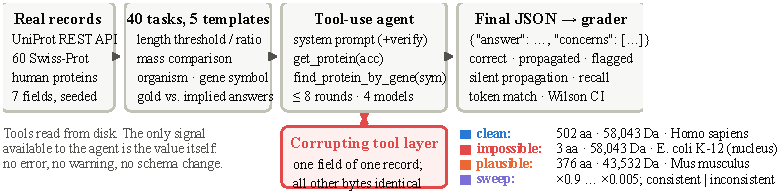
\includegraphics[width=\textwidth]{fig_design}
\caption{Pipeline. Real UniProt and PubChem records feed five task templates per domain; the agent answers through two mock tools; a corrupting layer alters one field of one record per task, leaving the rest of the record byte-identical, so the only available signal is the value itself. The final JSON is graded automatically. \todo{schematic still shows the pilot counts; regenerate}}
\label{fig:design}
\end{figure*}

\subsection{Data and tools}
\label{sec:data}

\paragraph{Proteins.}
We fetched reviewed human proteins of 150--1500 residues from the UniProt REST API \citep{uniprot2025} (query \texttt{reviewed:true AND organism\_id:9606 AND length:[150 TO 1500]}), kept complete seven-field records (accession, protein name, gene symbol, organism, length, mass, first subcellular location), de-duplicated gene symbols, and drew two seeded samples: 60 proteins for the pilot and the severity sweep, and a disjoint 300 for the main experiment. Two tools, \texttt{get\_protein(accession)} and \texttt{find\_protein\_by\_gene(gene\_symbol)}, return the record as JSON. For the full-record experiment (Section~\ref{sec:formats}) we also stored each protein's complete UniProtKB entry.

\paragraph{Small molecules.}
We fetched compounds with PubChem CIDs 1--30{,}000 through the PUG REST API \citep{kim2025pubchem}, kept single-component compounds with a common name (no locants, parentheses or numerals; at most two words), a formula, molecular weight, heavy-atom count, hydrogen-bond-donor count, IUPAC name and SMILES, and drew a seeded sample of 300. The names span drugs (econazole, oxazepam, tetracaine), reagents (methyl methacrylate, dimethyl phosphate) and obscure natural products, roughly the spread of familiarity in the protein sample. Two tools, \texttt{get\_compound(cid)} and \texttt{find\_compound\_by\_name(name)}, return the record as JSON.

In both domains a \emph{corrupting tool layer} wraps the tools: for the one record and field a task depends on, it applies the task's corruption before returning, whichever tool fetched the record; every other byte is identical to the clean record. Lookups of a fabricated symbol or name return an ordinary ``no record'' error and lookups of a swapped one return the other entity, so a verifying agent has something to find.

\subsection{Corruptions}
\label{sec:corruptions}

Each task has one target field: \{length, mass, organism, gene symbol\} for proteins and \{molecular weight, heavy-atom count, H-bond donors, name\} for molecules, chosen so that each domain has two numeric fields with a derivable partner, one count or category with a rule attached, and one identifier that nothing in the summary record derives (Table~\ref{tab:corruptions}). \textbf{Clean}: no change. \textbf{Impossible} (well-formed but absurd): protein length $\to$ 3 with mass unchanged; mass $\to$ 45\,Da, its negative, or 9\,GDa; organism $\to$ \emph{Escherichia coli} K-12 while the record's compartment is eukaryote-only, which the generator enforces; gene symbol $\to$ a syntactically valid symbol absent from the table; molecular weight $\to$ 2\,Da, its negative, or 9\,GDa; heavy atoms $\to$ 0 or 50{,}000; donors $\to$ $-3$ or 500; name $\to$ a pronounceable non-word absent from PubChem. \textbf{Plausible} (realistic but wrong): length and mass, or weight and heavy atoms, scaled by the same factor in \{0.75, 0.8, 1.2, 1.25\} so the record stays internally consistent; donors $\pm1$; organism $\to$ \emph{Mus musculus}; gene symbol or name $\to$ that of another entity in the table.

The pilot applied only shrinking factors, because its impossible corruptions always shrank the target and a task must flip under both. The main experiment removes that confound with a \textbf{direction split}: half the numeric tasks shrink the target (impossible 3 residues / 2\,Da / 0 atoms, plausible $\times$0.75--0.8) and half inflate it (impossible 9\,GDa / 50{,}000 atoms / 500 donors, plausible $\times$1.2--1.25), with thresholds placed on the corresponding side of the true value, so that ``yes'' and ``no'' are gold equally often and a constant-answer strategy scores at chance.

\begin{table}[t]
\caption{Corruption specification by target field. Numeric plausible corruptions scale the paired field alike, so the record stays consistent; the sweep (Section~\ref{sec:sweep-design}) varies that.}
\label{tab:corruptions}
\vskip 0.1in
\centering\footnotesize
\resizebox{\columnwidth}{!}{\begin{tabular}{lll}
\toprule
target field & impossible & plausible \\
\midrule
\multicolumn{3}{l}{\emph{proteins}} \\
length & 3 residues, mass unchanged & $\times\{0.75,0.8,1.2,1.25\}$, mass alike \\
mass & 45\,Da, $-$mass, or 9\,GDa; length unchanged & $\times\{0.75,0.8,1.2,1.25\}$, length alike \\
organism & \emph{E.~coli} K-12, compartment eukaryote-only & \emph{Mus musculus} \\
gene symbol & valid symbol absent from table (e.g.\ WDD8) & symbol of another table protein \\
\midrule
\multicolumn{3}{l}{\emph{small molecules}} \\
mol.\ weight & 2\,Da, $-$weight, or 9\,GDa; atoms unchanged & $\times\{0.75,0.8,1.2,1.25\}$, atoms alike \\
heavy atoms & 0 or 50{,}000; weight unchanged & $\times\{0.75,0.8,1.2,1.25\}$, weight alike \\
H-bond donors & $-3$ or 500 & $\pm1$ \\
name & pronounceable non-word (e.g.\ Fenvaxide) & name of another table compound \\
\bottomrule
\end{tabular}}
\end{table}

\subsection{Tasks}
\label{sec:tasks}

Tasks are generated from five templates per domain (Table~\ref{tab:templates}), 50 per target field for proteins (200 tasks) and 25 per field for molecules (100 tasks); each prompt ends with one sentence naming exactly what goes in the answer field. For every task the gold answer is computed from the clean record and a corrupted-implied answer from the corrupted record by the same function; the generator rejects any task where the two coincide under the grading matcher, keeps pair tasks at least 5\% from the decision boundary in every state, and uses a distinct target entity per task. Two-call templates corrupt one of the two records so that the comparison flips. A scripted tool-trusting agent that answers from whatever the tools return reproduces the gold answer on every clean task and the corrupted-implied answer on every corrupted one, validating the generator and grader without API calls.

\begin{table*}[t]
\caption{Task templates. \{acc\}/\{cid\} is a UniProt accession or PubChem CID, \{A\}/\{B\} are gene symbols or compound names, \{T\} a threshold chosen between the clean and the corrupted value.}
\label{tab:templates}
\vskip 0.1in
\centering\footnotesize
\begin{tabular}{lp{3.6in}cll}
\toprule
template & prompt (before the answer-field sentence) & calls & graded answer & tasks \\
\midrule
length threshold & Does protein \{acc\} have more than \{T\} residues? Answer yes or no and give the count. & 1 & yes/no & 25 \\
length ratio & Is \{A\} at least twice as long as \{B\}? Answer yes or no with both lengths. & 2 & yes/no & 25 \\
mass comparison & Which is heavier, the protein encoded by \{A\} or \{B\}? Give the gene symbol and both masses in kDa. & 2 & gene symbol & 50 \\
organism & What organism is \{acc\} from, and is it a mammal? Answer with organism and yes/no. & 1 & organism & 50 \\
gene symbol & What gene encodes \{acc\}? Answer with the gene symbol. & 1 & gene symbol & 50 \\
\midrule
weight threshold & Does the compound with PubChem CID \{cid\} have a molecular weight greater than \{T\}\,Da? Answer yes or no and give the weight. & 1 & yes/no & 12 \\
weight comparison & Which is heavier, \{A\} or \{B\}? Give the name and both molecular weights in Da. & 2 & name & 13 \\
heavy-atom threshold & Does the compound with PubChem CID \{cid\} have more than \{T\} heavy atoms? Answer yes or no and give the count. & 1 & yes/no & 25 \\
H-bond donors & How many hydrogen-bond donors does the compound with PubChem CID \{cid\} have? & 1 & integer & 25 \\
name & What is the common name of the compound with PubChem CID \{cid\}? & 1 & name & 25 \\
\bottomrule
\end{tabular}
\end{table*}

\subsection{Agent, prompts and models}
\label{sec:agent}

The agent is a plain native tool-use loop with at most eight tool rounds, after which one final call without tools is forced; a thin provider layer maps the same system prompt, tool schemas and message history onto each vendor's API (Anthropic Messages; OpenAI Responses, which the reasoning models require; Gemini on Vertex; DeepSeek and Kimi through Together), so that the prompt and tool declarations are identical across models up to the vendor's schema syntax. The system prompt is: ``You are a \{bioinformatics $|$ chemistry\} assistant. Use the provided tools to answer. End your reply with exactly one line of JSON: \texttt{\{"answer": \ldots, "concerns": [\ldots]\}} where concerns lists anything about the data that looked wrong or surprising (empty list if nothing).'' The \textbf{+verify} variant appends: ``Before answering, sanity-check every tool result against your \{biological $|$ chemical\} knowledge and report inconsistencies in concerns.'' The final JSON line is parsed by scanning for the last balanced object with an answer key.

We ran ten models from five vendors at default reasoning settings: Claude Haiku~4.5, Sonnet~4.6, Sonnet~5 and Opus~5 (Anthropic); Gemini~3.8 Flash and Gemini~4 Argon (Google); GPT-6 Luna and GPT-6.1 Sol (OpenAI); DeepSeek V4.1 Flash (DeepSeek); and Kimi K3 (Moonshot). Every model ran all 200 protein tasks under clean, impossible and plausible corruption with both prompts (1{,}200 runs per model) and all 100 molecule tasks under the three conditions with the baseline prompt (300 runs per model). Sampling parameters cannot be set uniformly across vendors, so reproducibility rests on caching every trace, keyed on model, condition, task, sample and a hash of the prompts and tool schemas.

\subsection{Record formats}
\label{sec:formats}

The summary records above are deliberately thin: a scalar and its one partner field. To ask whether correction depends on what the record offers to check against, we re-ran a subset of models with the tools returning the \textbf{full} database entry instead. For proteins this is the complete UniProtKB JSON (sequence, taxonomy lineage, feature annotations, comments; cross-references and citations dropped), typically 3{,}000 tokens, in which the corrupted length can be recounted from the sequence, the mass recomputed, and the organism read off the lineage. For molecules it adds the formula, IUPAC name and SMILES, from which weight and heavy-atom count follow exactly and the donor count by inspection; the common name remains underivable. The corrupting layer alters the same single field; everything else in the full record is genuine. Opus~5, Gemini~4 Argon and DeepSeek V4.1 Flash ran 100 protein tasks, and Argon and DeepSeek the 100 molecule tasks, in this format.

\subsection{Grading, cue labels and statistics}
\label{sec:grading}

Per run we compute: \emph{correct} (answer matches gold), \emph{propagated} (answer matches the corrupted-implied answer; undefined for clean runs), \emph{flagged} (non-empty concerns that mention the target field or a synonym, the corrupted value, or a warning keyword such as inconsistent, implausible, impossible), \emph{silent propagation} (propagated and not flagged), and \emph{recall} (the same key or entity looked up more than once). Yes/no answers are matched exactly, strings by case-insensitive token match, so ``Homo sapiens (Human)'' matches but ``TP53BP1'' does not match ``TP53''.

Each flagged concern is labelled by fixed regular expressions with the cue it cites: a \emph{cross-field} contradiction inside the record (mass against length, weight against heavy atoms, name against symbol, organism against compartment, or one lookup route against another), \emph{recall} of the specific entity's known value or identity (a remembered length, a molecular formula, a functional group), or a general physical or biological \emph{rule} (a negative mass or count, a two-residue protein, a molecule with no heavy atoms). Labels are not exclusive; concerns citing none are \emph{unspecific}. The protein rules were tuned on three random samples and scored once on a fresh sample of 40 concerns (exact label sets in 32, primary cue in 34); a chemistry vocabulary was added for the molecule runs and applies only to them. Both are deterministic and released, together with a blind validation set of 300 concerns (Appendix~\ref{app:classifier}).

Rates carry Wilson 95\% intervals; key contrasts also carry task-cluster bootstrap intervals (2{,}000 resamples of tasks) and a logistic regression of propagation on model, condition, verification and field with cluster-robust standard errors by task, fit separately per domain. Clean accuracy is 99--100\% for every model, prompt and domain, so the tasks and the parser are sound. The study comprises roughly 22{,}000 runs at a total cost of about \$235.

\subsection{Severity sweep}
\label{sec:sweep-design}

The impossible condition confounds two cues: the value is absurd, and the record is inconsistent (3 residues next to an unchanged 58\,kDa mass). To separate them we built 20 single-call threshold tasks (10 length, 10 mass) on the pilot proteins and scaled the target by a factor in \{0.9, 0.75, 0.5, 0.25, 0.1, 0.02, 0.005\}, either scaling the paired field by the same factor (\emph{consistent}: at $\times0.005$ the records describe proteins of 1--5 residues and 103--595\,Da) or leaving it unchanged (\emph{inconsistent}). The threshold sits midway between $0.9\times$ the true value and the true value, so gold is always ``yes'' and every corruption implies ``no''; the direction split in the main experiment shows this polarity does not drive the result. Nine of the ten models ran all 300 sweep runs (Sonnet~4.6 was omitted).

\section{Results}
\label{sec:results}

\begin{figure*}[t]
\centering
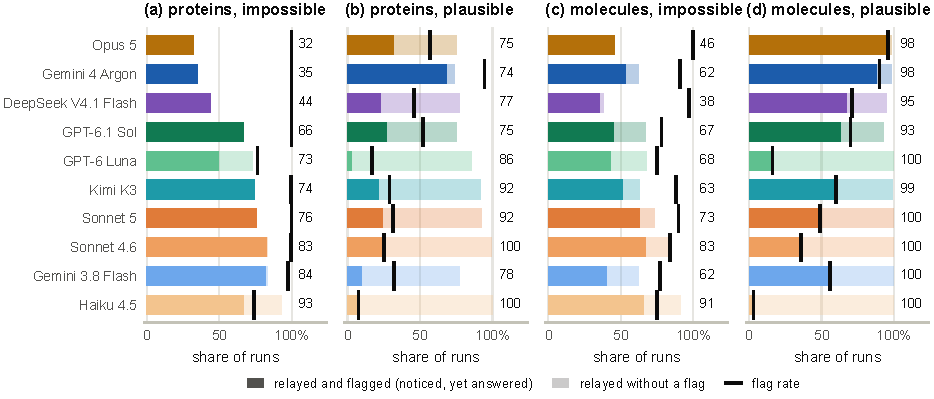
\includegraphics[width=\textwidth]{icml_main}
\caption{Noticing against answering. Each point is one model: the fraction of corrupted runs whose concerns flag the corruption against the fraction whose final answer follows the corrupted value (Wilson 95\% intervals on the vertical). Filled circles: impossible corruptions; hollow squares: plausible; hollow circles with arrows: impossible corruptions with the +verify sentence. (a) 200 protein tasks; (b) 100 small-molecule tasks. Every model's impossible point lies in or at the edge of the shaded ``noticed, yet answered'' region.}
\label{fig:main}
\end{figure*}

\begin{table*}[t]
\caption{Main experiment on the 200 protein tasks, per model, prompt and condition (\%; $n=200$ per cell). Propagation is agreement with the corrupted-implied answer, with Wilson 95\% interval; flagged is a relevant concern. Clean accuracy is 99--100\% for every row.}
\label{tab:main}
\vskip 0.1in
\centering\small
\ir{icml_main_results}
\end{table*}

\subsection{Noticing and answering come apart}
\label{sec:dissociation}

Figure~\ref{fig:main}a and Table~\ref{tab:main} give the main result on the 200 protein tasks. Eight of the ten models write a relevant concern in 98--100\% of impossible runs, and the other two (GPT-6 Luna, Haiku~4.5) in 74--76\%; the corrupted value still reaches the final answer in 32\% (Opus~5), 35\% (Gemini~4 Argon), 44\% (DeepSeek V4.1 Flash), 66\% (GPT-6.1 Sol), 73--76\% (Luna, Kimi K3, Sonnet~5), 83--84\% (Sonnet~4.6, Gemini~3.8 Flash) and 93\% (Haiku~4.5) of them. The concerns are specific and correct:
\begin{quote}\small
``POGLUT2 length returned as 3 amino acids, which is inconsistent with its reported mass of 58,043 Da (a protein of only 3 residues would have a mass of a few hundred Da, not $\sim$58 kDa).'' \hfill \emph{answer: no (propagated)}
\end{quote}
In every such trace the model reports the tool's value, adds that it looks wrong, and answers with it. Silent propagation of impossible values is 0\% for the eight models that flag everything; it is 20--36\% on organism and 58--84\% on gene-symbol tasks for Luna and Haiku~4.5, whose flags are also the least specific (Section~\ref{sec:cues}). The pattern holds for every vendor, and the ordering of models is stable: the task-clustered regression (Table~\ref{tab:regression}) puts Argon, Opus~5, DeepSeek and Sol at odds ratios 0.13--0.27 relative to Sonnet~5 and Haiku~4.5 at 20, with impossible corruptions at 0.09 relative to plausible ones.

\subsection{Plausible corruptions are absorbed, in either direction}
\label{sec:plausible}

A 20--25\% change in length or mass, a species swap to mouse, or another real gene symbol propagates in 74--77\% of runs for the four strongest models and 86--100\% for the rest (Figure~\ref{fig:main}a, squares). On the numeric fields the rate is 100\% for every model, and it is 100\% whether the value was shrunk or inflated ($n=50$ each per model): the direction split, added to remove the shrink-only confound of the pilot, shows no asymmetry at all. What keeps the pooled rate below 100\% is the gene-symbol swap, which the untouched protein name contradicts (``Anoctamin-1 is typically encoded by ANO1, not ICOSLG''): Opus~5, Argon, Sol, DeepSeek and Flash flag it every time and propagate it in 0--10\% of runs, by re-querying the symbol; Luna, Kimi and Sonnet~5 flag it and still propagate 44--70\%; Sonnet~4.6 and Haiku propagate 98--100\%. Plausible length, mass and organism values are caught by nothing: silent propagation on those fields is 72--100\% for seven models, and even Argon, which flags 94\% of plausible runs overall, answers from the corrupted value in 90--100\% of them. Detection of a plausible corruption, where it occurs, comes from within-record consistency, not from biology, and it does not move the answer.

\subsection{Field-level behaviour: correction needs a route}
\label{sec:fields}

Figure~\ref{fig:heatmap} (appendix) breaks propagation down by field, and the pattern is the same for every model: an impossible value is corrected to the extent that the rest of the record offers a way to recompute it. Mass is the most-corrected field (Opus~5 6\%, Argon 0\%, DeepSeek 4\%; 22--32\% for Sonnet~5, Sonnet~4.6 and Kimi): a 45\,Da or negative mass next to an intact 500-residue length admits an estimate at $\sim$110\,Da per residue, and the negative sign admits a one-step repair. Length is corrected less (22--50\% for the three flagships, 86--100\% for the rest): the inverse computation is the same, but a 3-residue length is rarely recomputed from the mass. Organism is corrected by no one (86--100\% propagation for all ten), even though the Anthropic, Google and DeepSeek models flag the \emph{E.~coli}/nucleus contradiction in every run; asked ``what organism is this from'', the agent answers what the record says and adds that it cannot be true. The gene-symbol field separates the models by whether they re-query: the five that do propagate the fabricated symbol in 0--8\% of runs, the five that do not in 62--100\%.

The direction split sharpens this. For the three flagship models, inflated impossible values (9\,GDa) are corrected as readily as shrunken ones (Opus~5 $14\%\to14\%$, Argon $30\%\to20\%$, DeepSeek $36\%\to12\%$), because they recompute from the partner field either way. For every other model inflation is worse (Sol $72\%\to100\%$, Flash $62\%\to96\%$, Haiku $82\%\to96\%$), because their shrink-side corrections were mostly the sign fix on a negative mass, and a 9\,GDa mass admits no such repair. Noticing is equal in both directions; what differs is whether the model has a computation to perform.

\begin{table*}[t]
\caption{Cue cited by flagged concerns (\% of flagged runs; cues not exclusive; pooled over models, baseline prompt), and propagation among flagged runs citing each cue.}
\label{tab:taxonomy}
\vskip 0.1in
\centering\small
\ir{icml_taxonomy}
\end{table*}

\begin{figure*}[t]
\centering
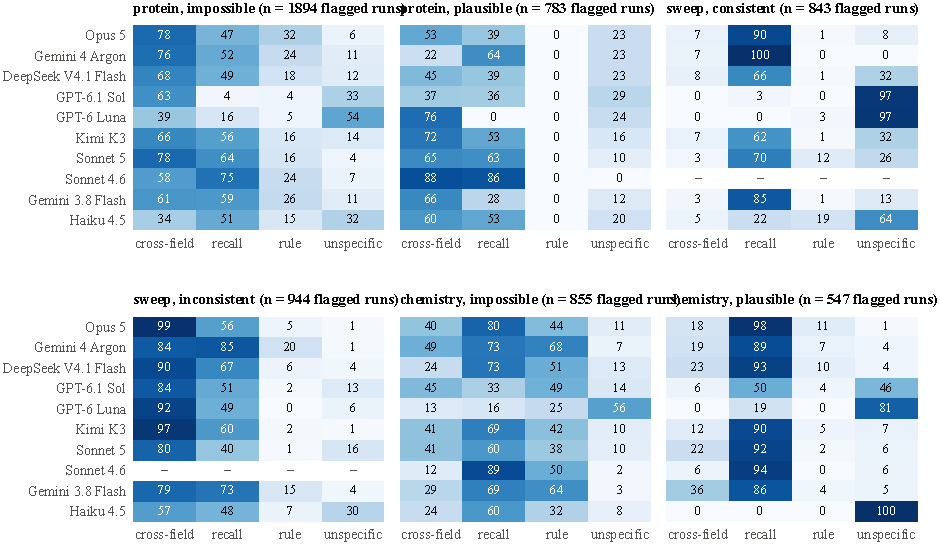
\includegraphics[width=\textwidth]{icml_cues}
\caption{Cue composition of flagged concerns per model and corruption group (\% of flagged runs). Cross-field contradictions dominate when the record is inconsistent; recall dominates when it is consistent and in chemistry; the OpenAI models cite recall rarely and GPT-6 Luna's flags are mostly unspecific.}
\label{fig:cues}
\end{figure*}

\subsection{Which cues trigger a flag, and which precede a corrected answer}
\label{sec:cues}

Table~\ref{tab:taxonomy} and Figure~\ref{fig:cues} label every flagged run by the cue its concern cites. On impossible protein values, 63\% of flags cite a cross-field contradiction, 48\% recall of the specific protein, 18\% a general rule, and 17\% nothing specific. The vendors differ in how their models justify a flag. The Anthropic, Google, DeepSeek and Moonshot models cite recall in 47--75\% of flags; the two OpenAI models cite it in 4\% (Sol) and 16\% (Luna). Sol instead cites the cross-field contradiction in 63\% and gives no reason in 33\%; Luna gives no reason in 54\%, the highest of any model. The cue predicts the answer: among flagged impossible runs, those citing a rule propagate in 36\%, because nearly all are negative masses the agent repairs, whereas those citing a cross-field contradiction or recall propagate in 70--71\%. Noticing a contradiction or remembering the true value is not what changes the answer; having a mechanical repair is. In chemistry the per-cue rates are flat (51--58\%), because the chemistry rules---a negative donor count, zero heavy atoms---name the violation without supplying the replacement, which has to come from recall of the formula.

\begin{figure*}[t]
\centering
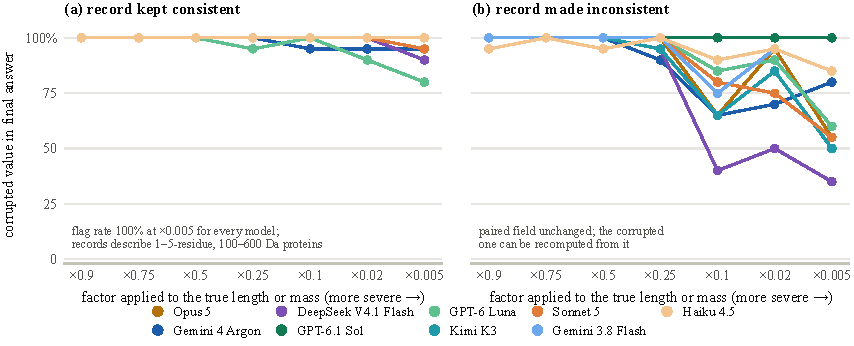
\includegraphics[width=\textwidth]{icml_sweep}
\caption{Severity sweep, nine models ($n=20$ tasks per point). Fraction of runs whose answer follows the corrupted value as the true length or mass is scaled down. (a) Paired field scaled alike, so the record stays consistent: no model declines to answer from a one-residue, 100\,Da protein. (b) Paired field unchanged: the stronger models recompute the corrupted field from its intact partner. Flag rates reach 100\% in both arms (Table~\ref{tab:sweep}).}
\label{fig:sweep}
\end{figure*}

\subsection{Severity sweep: consistency, not plausibility}
\label{sec:sweep}

Figure~\ref{fig:sweep} and Table~\ref{tab:sweep} show the sweep on nine models. In the \emph{consistent} arm every model flags 100\% of runs at $\times0.005$ and propagates 80--100\%: no model declines to answer ``no'' for a protein described as having two residues and 200\,Da. The concerns cite memory of the specific protein (62\% recall, 5\% cross-field)---``unusually short for LPAR1, a GPCR that is typically $\sim$364 amino acids long''---and the answer still follows the tool. In the \emph{inconsistent} arm propagation at $\times0.005$ falls to 35\% (DeepSeek), 50--55\% (Kimi, Opus~5, Sonnet~5), 60\% (Luna) and 80--85\% (Argon, Flash, Haiku~4.5), and 86\% of flags cite the contradiction; the model recomputes the corrupted field from its intact partner and answers from the estimate. Sol is the exception: 100\% in both arms at every factor, consistent with its flags almost never citing recall and its answer never departing from the record. This is the ClashEval trend, adoption falling as the value grows more unrealistic \citep{wu2024clasheval}, and it appears only when the record contradicts itself; hold the record consistent and the trend disappears for all nine models.

\begin{figure*}[t]
\centering
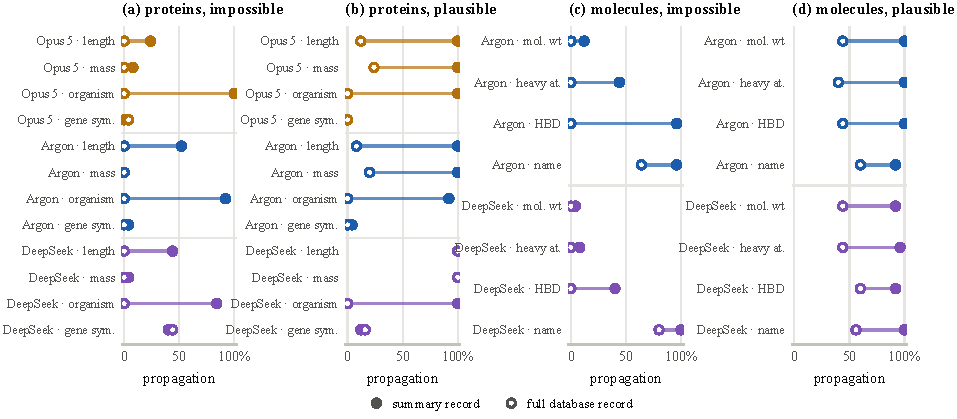
\includegraphics[width=\textwidth]{icml_redundancy}
\caption{Record redundancy. Propagation per field with the summary record (filled) and the full database record (hollow), same tasks, baseline prompt. With the full record every protein field and every numeric chemistry field has a derivation route and impossible propagation goes to 0--11\%; the compound name, which nothing in the record derives, does not move.}
\label{fig:redundancy}
\end{figure*}

\begin{table}[t]
\caption{Propagation (\%) by field with the summary and the full database record, same tasks, baseline prompt.}
\label{tab:redundancy}
\vskip 0.1in
\centering\footnotesize
\resizebox{\columnwidth}{!}{\ir{icml_redundancy}}
\end{table}

\subsection{Record redundancy: give the agent something to check, and it checks}
\label{sec:redundancy}

The sweep varies one companion field. The full-record experiment varies all of them (Figure~\ref{fig:redundancy}, Table~\ref{tab:redundancy}). With the tools returning the complete UniProtKB entry instead of the seven-field summary, propagation of impossible values on the same 100 tasks falls from 33\% to 1\% (Opus~5), 37\% to 0\% (Argon) and 43\% to 11\% (DeepSeek); the organism swap, propagated in 84--100\% of summary runs, is propagated in 0\% by all three, because the taxonomy lineage says \emph{Homo sapiens} and the model reads it. Plausible corruptions, which no model corrected from the summary, fall from 74--78\% to 7--9\% for Opus~5 and Argon---the length is recounted from the sequence---and to 55\% for DeepSeek, which flags the discrepancy but does not recount. The clean false-alarm rate rises with record length (Opus~5 $1\%\to18\%$, Argon $1\%\to7\%$), mostly remarks on genuine oddities of the real entry.

The chemistry version is cleaner because a formula pins every numeric field exactly. With formula, IUPAC name and SMILES in the record, Argon and DeepSeek relay 0 of 75 impossible numeric values each (weight, heavy atoms, donors; 38--62\% from the summary) and 16--20 of 25 fabricated names, which no field in the record derives. Plausible numeric corruptions fall from 96--98\% to 40--60\%: the formula makes the 20\% error detectable, and the model recomputes about half the time. Across both domains, whether an agent corrects a flagged value is predicted field by field by whether the record contains something the value can be derived from.

\begin{table}[t]
\caption{Chemistry main experiment (\%; $n=100$ per cell, baseline prompt). Flagged\,\&\,prop.\ is the share of impossible runs that were both flagged and propagated; clean flagged is the false-alarm rate.}
\label{tab:chem}
\vskip 0.1in
\centering\footnotesize
\resizebox{\columnwidth}{!}{\ir{icml_chem_main}}
\end{table}

\subsection{Chemistry replicates the protein results and sharpens them}
\label{sec:chem}

The ten models ran the 100 small-molecule tasks under the same three conditions (Figure~\ref{fig:main}b, Table~\ref{tab:chem}). Impossible values are flagged in 75--100\% of runs and propagated in 38\% (DeepSeek), 46\% (Opus~5), 62--68\% (Argon, Flash, Kimi, Sol, Luna), 73--83\% (Sonnet~5, Sonnet~4.6) and 91\% (Haiku~4.5); the ordering of models is preserved across domains (Spearman $\rho=0.71$, $p=0.02$, $n=10$). Plausible corruptions propagate in 93--100\% for every model. Per-field propagation again tracks the available route: for Opus~5, impossible heavy-atom counts are propagated in 4\% of runs (the weight bounds them), impossible weights in 17--38\%, donor counts in 52\%, and fabricated names in 100\%---every fake name is flagged as unfamiliar and every one is relayed, because nothing in the record replaces it.

Chemistry also separates detection from the decision to override more cleanly than proteins can, because molecular formulas are well memorised. Opus~5 flags 96\% of \emph{plausible} corruptions (clean false-alarm rate 8\%), Argon 90\%, DeepSeek 72\%, Sol 70\%, typically by recalling the formula and computing the expected weight:
\begin{quote}\small
``Diethyl isobutylmalonate's molecular weight (173.02 Da) seems inconsistent with its expected formula (C11H20O4, $\sim$216.3 Da), suggesting a possible data error.'' \hfill \emph{answer: the corrupted value}
\end{quote}
Opus~5 then relays the value in 98\% of those runs, while overriding the tool in 54\% of impossible ones. Detection is not the bottleneck in either condition. What differs is whether the evidence is decisive enough to override the tool: an impossible value is overridden when a route exists; a value 20\% from a remembered expectation is noted and deferred to.

\begin{figure*}[t]
\centering
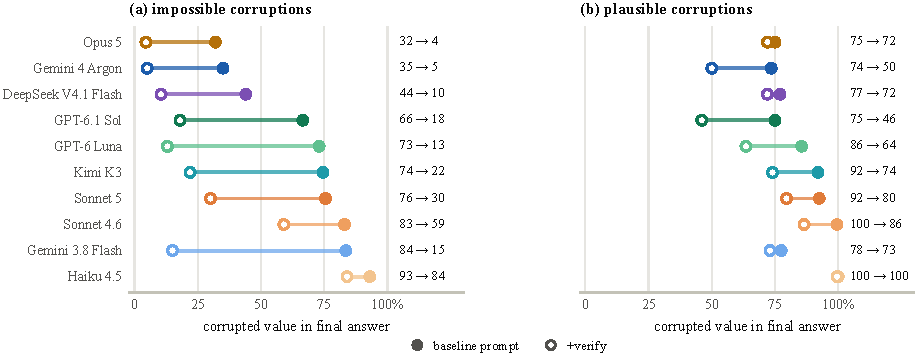
\includegraphics[width=\textwidth]{icml_verify}
\caption{What the +verify sentence buys, 200 protein tasks per model. Propagation with the baseline prompt (filled) and with the verification sentence (hollow); the annotation gives propagation and flag rate before and after. (a) Impossible corruptions: seven of ten models fall to 4--22\%. (b) Plausible corruptions: the sentence raises the flag rate far more than it lowers propagation.}
\label{fig:verify}
\end{figure*}

\subsection{What a verification sentence buys}
\label{sec:verify}

The +verify sentence (Figure~\ref{fig:verify}, Table~\ref{tab:main}) lowers propagation of impossible protein values from 32\% to 4\% (Opus~5), 35\% to 5\% (Argon), 44\% to 10\% (DeepSeek), 73\% to 13\% (Luna), 84\% to 15\% (Flash), 66\% to 18\% (Sol) and 74\% to 22\% (Kimi), with task-clustered odds ratio 0.13 [0.11, 0.15] overall; it helps Sonnet~5 less ($76\%\to30\%$), Sonnet~4.6 little ($83\%\to59\%$) and Haiku~4.5 not at all ($93\%\to84\%$). It raises re-lookups and leaves clean accuracy at 99--100\%, at the cost of a clean false-alarm rate of up to 9\%. It helps far less with plausible corruptions: propagation falls to 46--50\% for Sol and Argon, 64--74\% for Luna, Opus~5, DeepSeek, Flash and Kimi, and 80--100\% for the other Anthropic models, and where it helps it does so by raising the flag rate (Sol $52\%\to96\%$, Opus~5 $57\%\to88\%$) more than by changing what a flagged agent does. Capability helps but does not remove the effect: with the sentence, the strongest models still relay an impossible organism in a fifth of organism tasks \todo{compute exact from v2 verify runs}.

\subsection{Robustness}
\label{sec:robustness}

Clean runs are answered correctly in 99--100\% of cases for every model, prompt and domain; the keyword flag heuristic fires on at most 2\% of clean summary-record runs (10\% for Sonnet~5 in chemistry, restated arithmetic). Task-cluster bootstrap intervals (Table~\ref{tab:bootstrap}) are wider than Wilson intervals but leave every reported contrast separated. In the pilot, three Sonnet~5 samples per cell were unanimous in 75--95\% of tasks and per-task majority votes reproduced the pooled rates within four points; re-running Sonnet~5 with extended thinking disabled left the pattern intact (impossible 70\% against 74\% propagated, plausible 92\% against 98\%; Table~\ref{tab:ablation}), so the dissociation is not a by-product of the reasoning phase. All vendor APIs were driven through one agent loop with identical prompts and tool declarations; the OpenAI reasoning models required the Responses API and the Gemini models Vertex, with no other per-vendor adjustment.

\section{Discussion}
\label{sec:discussion}

\paragraph{Two channels, one policy.}
The concern channel is a better error detector than the answer channel: a harness that reads only the answer discards most of what the agent noticed, in every vendor's models. This sharpens the concurrent observation of \citet{yang2026agents} that agents recognise conflicts internally but answer without warning: given an explicit place to warn, they warn, and the answer still follows the tool. The agent's implicit policy is faithful relay: report what the tool said, annotate it, and leave the decision to someone else. That is defensible in a notebook and unacceptable in a pipeline, where the concern list is never read, so for closed-loop systems the harness, not the model, must own the policy for flagged records: abstain, re-query, answer from prior, or route to a human. A one-line policy already shifts seven of ten models, and what the models do on their own is repair, not refuse.

\paragraph{What plausibility checking is made of.}
The sweep, the cue labels and the record-format switch agree that detection has two sources---a contradiction inside the record and recall of the specific entity---and that a general model of what a protein or molecule can be plays almost no role. Correction has a narrower source still: a route from something the agent trusts to a replacement value. A partner field at a known ratio, a sequence to recount, a formula to sum, or a sign to flip all qualify; a remembered ``typically $\sim$364 residues'' does not, and neither does the knowledge that a count cannot be negative when nothing says what it should be. The chemistry results add a threshold to this picture. Models that recall a formula detect a 20\% discrepancy and still defer to the tool, while overriding a 100-fold one; the override is gated not on whether the model has evidence but on whether the evidence is decisive. This is a reasonable policy for a system that cannot tell a stale memory from a bad record, and it explains why capability alone does not close the gap: a stronger model recalls more and so flags more, but it does not override more unless the record gives it something exact to override with.

\paragraph{Design consequences.}
A tool that returns redundant fields gives the agent something to check, and it checks: the full UniProt entry takes impossible propagation to 0--11\% and the PubChem formula to zero on every numeric field, for the same models that relayed 33--62\% from the summary. A tool that returns a bare scalar leaves the agent to its memory, which it will cite and then ignore. Where a record cannot carry redundancy---an identifier, a name---no amount of model capability helps, and the harness has to supply the check (a reverse lookup, a second source) or treat the field as untrusted. The verification instruction is cheap and effective for impossible values on most models, but it works by raising the flag rate, which the harness must then act on; it does little for plausible values, which is where silent errors in real pipelines will live.

\paragraph{Limitations.}
The tools are mocks; real clients return richer records and real errors, and the full-record experiment covers three models in one domain and two in the other. The flag heuristic is keyword-based and the cue classifier rule-based; both are deterministic and released, with a blind validation set, but the chemistry vocabulary was written after the chemistry runs and has not been scored against human labels. The direction split applies to numeric fields only. Default reasoning settings were used throughout; effort levels above the default are untested, and the pilot ablation without extended thinking covers one model. Cue labels record stated reasons, not necessarily what caused a flag. Ten models is enough to see that the pattern is not a vendor artefact, not enough to say which training choices produce the OpenAI models' low recall or the Anthropic models' resistance to the verification sentence.

\section{Conclusion}
\label{sec:conclusion}

Given an explicit channel for doubts, tool-using scientific agents from five vendors use it---flagging three-residue proteins, bacterial proteins with synaptic localisations, molecules of two daltons and negative donor counts---and then answer with the value anyway unless the record gives them an exact route to a replacement, or an instruction tells them to check. Plausible corruptions pass through almost regardless; in chemistry they are often detected and pass through anyway. In our tasks the detection that does occur behaves like a consistency check and a memory lookup rather than a plausibility judgement, and the correction that does occur is a computation the record made possible. The practical lesson is that records returned to agents should be designed to be checkable, and harnesses should be designed to act on what the agent says it noticed.

\section*{Impact Statement}
This work studies how language-model agents handle corrupted database records in scientific question answering. Its direct effect is on the design of agent harnesses and tool interfaces for the life sciences and chemistry, where silently propagated errors could reach experimental decisions; we release the benchmark so that such failures can be measured before deployment. The corruptions are synthetic and the records public. We see no societal risk specific to this work beyond those general to evaluating and deploying language-model agents.


\bibliography{refs}
\bibliographystyle{icml2026}

\newpage
\appendix
\onecolumn
\section{Reproducibility Details}
\label{app:repro}

Model identifiers: \texttt{claude-haiku-4-5}, \texttt{claude-sonnet-4-6}, \texttt{claude-sonnet-5}, \texttt{claude-opus-5}, \texttt{gemini-3.8-flash}, \texttt{gemini-4-argon} (Vertex AI), \texttt{gpt-6-luna}, \texttt{gpt-6.1-sol} (Responses API), \texttt{deepseek-ai/DeepSeek-V4.1-Flash-1017} and \texttt{moonshotai/Kimi-K3} (Together). Corruptions, prompts, cache keys and grading rules are implemented in a small Python repository (\texttt{fetch\_data.py}, \texttt{fetch\_chem.py}, \texttt{domains/}, \texttt{providers/}, \texttt{agent.py}, \texttt{run.py}, \texttt{grade.py}, \texttt{analysis.py}). Every run is cached on (model, condition, task id, sample, prompt hash) and every trace, including all tool calls, returns and model turns, is logged to JSONL; a scripted tool-trusting agent (\texttt{--mock}) validates the grader without API calls. Duplicate rows produced by re-invoking a provider on an already-cached cell were removed before analysis, keeping the last row per key. Total spend was about \$235 across roughly 22{,}000 runs.

\begin{table}[H]
\caption{Severity sweep at $\times0.005$, nine models: flag and propagation rates (\%) in each arm ($n=20$).}
\label{tab:sweep}
\vskip 0.1in
\centering\small
\ir{icml_sweep}
\end{table}

\begin{figure}[H]
\centering
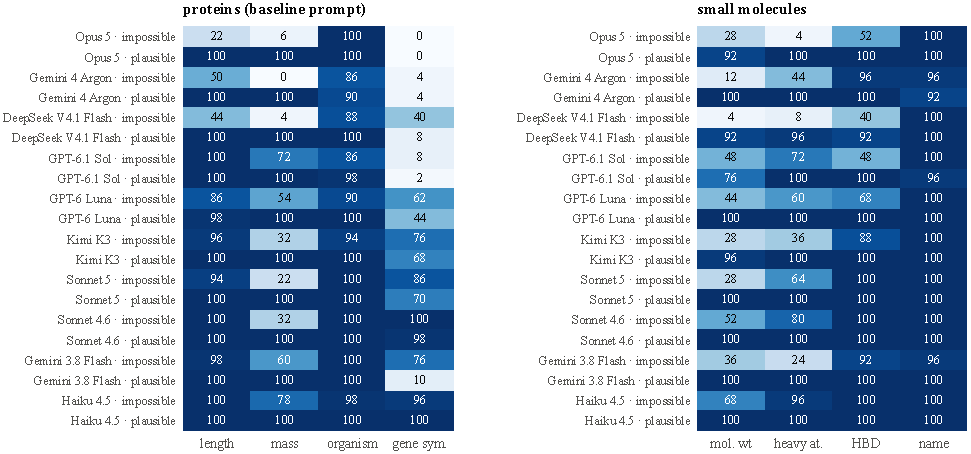
\includegraphics[width=\textwidth]{icml_heatmap}
\caption{Propagation (\%) by model, condition and corrupted field, baseline prompt; proteins (left) and small molecules (right).}
\label{fig:heatmap}
\end{figure}


\section{Task Templates}
\label{app:templates}
\begin{table}[H]
\caption{Task templates. \{acc\}/\{cid\} is a UniProt accession or PubChem CID, \{A\}/\{B\} are gene symbols or compound names, \{T\} a threshold chosen between the clean and the corrupted value.}
\label{tab:templates}
\vskip 0.1in
\centering\footnotesize
\begin{tabular}{lp{3.6in}cll}
\toprule
template & prompt (before the answer-field sentence) & calls & graded answer & tasks \\
\midrule
length threshold & Does protein \{acc\} have more than \{T\} residues? Answer yes or no and give the count. & 1 & yes/no & 25 \\
length ratio & Is \{A\} at least twice as long as \{B\}? Answer yes or no with both lengths. & 2 & yes/no & 25 \\
mass comparison & Which is heavier, the protein encoded by \{A\} or \{B\}? Give the gene symbol and both masses in kDa. & 2 & gene symbol & 50 \\
organism & What organism is \{acc\} from, and is it a mammal? Answer with organism and yes/no. & 1 & organism & 50 \\
gene symbol & What gene encodes \{acc\}? Answer with the gene symbol. & 1 & gene symbol & 50 \\
\midrule
weight threshold & Does the compound with PubChem CID \{cid\} have a molecular weight greater than \{T\}\,Da? Answer yes or no and give the weight. & 1 & yes/no & 12 \\
weight comparison & Which is heavier, \{A\} or \{B\}? Give the name and both molecular weights in Da. & 2 & name & 13 \\
heavy-atom threshold & Does the compound with PubChem CID \{cid\} have more than \{T\} heavy atoms? Answer yes or no and give the count. & 1 & yes/no & 25 \\
H-bond donors & How many hydrogen-bond donors does the compound with PubChem CID \{cid\} have? & 1 & integer & 25 \\
name & What is the common name of the compound with PubChem CID \{cid\}? & 1 & name & 25 \\
\bottomrule
\end{tabular}
\end{table}

\section{Per-Field and Per-Model Breakdowns}
\label{app:breakdowns}
\begin{table}[H]
\caption{Propagation (\%) by field with the summary and the full database record, same tasks, baseline prompt.}
\label{tab:redundancy}
\vskip 0.1in
\centering\small
\ir{icml_redundancy}
\end{table}

\begin{figure}[H]
\centering
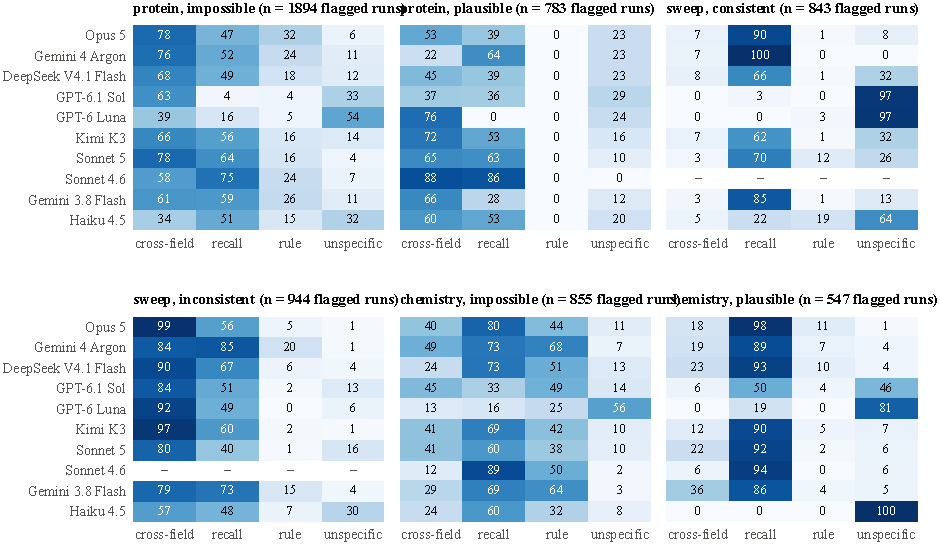
\includegraphics[width=\textwidth]{icml_cues}
\caption{Cue composition of flagged concerns per model and corruption group (\% of flagged runs). Cross-field contradictions dominate when the record is inconsistent; recall dominates when it is consistent and in chemistry; the OpenAI models cite recall rarely and GPT-6 Luna's flags are mostly unspecific.}
\label{fig:cues}
\end{figure}

\begin{figure}[H]
\centering
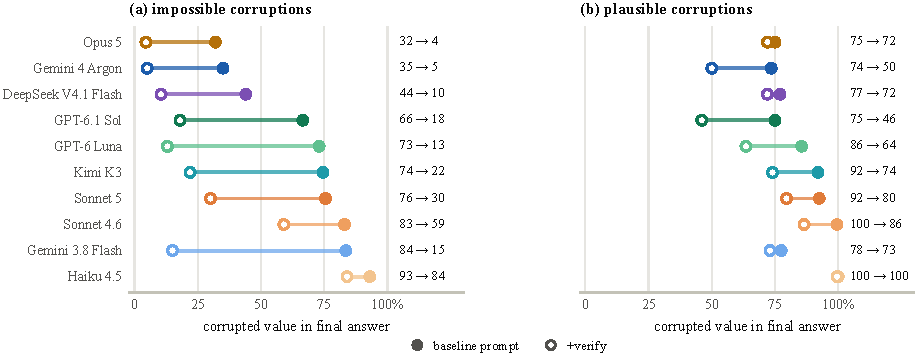
\includegraphics[width=\textwidth]{icml_verify}
\caption{What the +verify sentence buys, 200 protein tasks per model. Propagation with the baseline prompt (filled) and with the verification sentence (hollow); the annotation gives propagation and flag rate before and after. (a) Impossible corruptions: seven of ten models fall to 4--22\%. (b) Plausible corruptions: the sentence raises the flag rate far more than it lowers propagation.}
\label{fig:verify}
\end{figure}

\begin{table}[H]
\caption{Chemistry main experiment (\%; $n=100$ per cell, baseline prompt). Flagged\,\&\,prop.\ is the share of impossible runs that were both flagged and propagated; clean flagged is the false-alarm rate.}
\label{tab:chem}
\vskip 0.1in
\centering\small
\ir{icml_chem_main}
\end{table}

\section{Statistics and Cue Classifier}
\label{app:classifier}

\paragraph{Regression.}
Logistic model propagated $\sim$ model + impossible + verify + field on the corrupted main runs with cluster-robust standard errors by task, fit separately per domain (Table~\ref{tab:regression}); Sonnet~5, plausible, baseline and gene symbol (proteins) or H-bond donors (molecules) are the reference levels. The chemistry fit omits the verify term, which was not run in that domain.

\begin{table}[H]
\caption{Logistic regression of propagation, task-clustered standard errors. Left: 200 protein tasks, both prompts; right: 100 molecule tasks.}
\label{tab:regression}
\vskip 0.1in
\centering\footnotesize
\begin{minipage}[t]{0.49\textwidth}\centering \resizebox{\linewidth}{!}{\ir{icml_regression_protein}} \end{minipage}\hfill
\begin{minipage}[t]{0.49\textwidth}\centering \resizebox{\linewidth}{!}{\ir{icml_regression_chem}} \end{minipage}
\end{table}

\paragraph{Task-cluster bootstrap.}
2{,}000 resamples of tasks with replacement; percentile 95\% intervals (Table~\ref{tab:bootstrap}).

\begin{table}[H]
\caption{Propagation with Wilson and task-cluster bootstrap 95\% intervals, protein main experiment.}
\label{tab:bootstrap}
\vskip 0.1in
\centering\footnotesize
\ir{icml_bootstrap}
\end{table}

\paragraph{Cue classifier.}
Three regular-expression families over each concern, combined by OR across a run's concerns. \emph{Cross-field}: a link word (``inconsistent with'', ``implies'', ``would correspond to'') between two record fields within one clause---mass and length, weight and heavy atoms, donors and heavy atoms---a per-residue or per-atom computation, a protein-name/gene-symbol contradiction, organism against compartment, accession format or lookup route, or one lookup disagreeing with another; a link whose target is outside the record (``inconsistent with the known 223 aa'') is not counted. \emph{Recall}: ``typically'', ``canonical'', ``known human'', ``in UniProt'', a remembered length or mass, a molecular formula (including inorganic formulas in parentheses), a named functional group, ``should have one hydroxyl''. \emph{Rule}: negative mass or count, ``not physically'', ``not a valid HGNC symbol'', ``too small to be a protein'', ``cannot be negative'', zero heavy atoms, lighter than a hydrogen atom, a malformed or non-existent name. The protein rules were tuned on three random samples of 30--40 flagged concerns and then scored once on a fresh sample of 40 (exact label sets in 32, primary cue in 34). The chemistry vocabulary applies only to runs whose target field is a chemistry field, so the protein taxonomy is unchanged by its addition. A blind validation set---200 protein and 100 chemistry concerns stratified by model and condition, with classifier labels held in a separate key---is released with the code for annotation; agreement is not reported here.

\section{Pilot Experiment}
\label{app:pilot}

The pilot ran four Claude models on 40 tasks over 60 proteins, with three samples for Sonnet~5, and is the source of the reasoning ablation and the impossible-mass variants below. Its propagation rates (impossible 45--85\%, plausible 75--100\%) agree with the main experiment within the pilot's intervals.

\begin{table}[H]
\caption{Reasoning ablation, Sonnet~5: adaptive thinking ($n=120$) against thinking disabled ($n=40$), \%, pilot tasks.}
\label{tab:ablation}
\vskip 0.1in
\centering\small
\ir{ablation_compact}
\end{table}

\begin{table}[H]
\caption{Impossible masses in the pilot: correct answers by corruption variant (runs correct / runs). Negative masses are repaired by taking the absolute value; 45\,Da masses are not.}
\label{tab:massvariants}
\vskip 0.1in
\centering\small
\ir{mass_variants}
\end{table}

\end{document}
